\documentclass{standalone}
\usepackage[T1]{fontenc}
\usepackage[utf8]{inputenc}
\usepackage{pgf,tikz}
\usepackage{pgfplots}
\pgfplotsset{compat=1.9}

\begin{document}

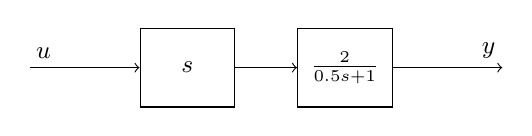
\begin{tikzpicture}[block/.style={rectangle, draw, minimum width=12mm, minimum height=10mm},
  sumnode/.style={circle, draw, inner sep=1pt},
  node distance=20mm]
  \small 
  \node[coordinate] (input) {};
  \node[block, right of=input] (D) {$s$};
  \node[block, right of=D] (G) {$\frac{2}{0.5s + 1}$};
  \node[coordinate, right of=G] (output) {};
 
  \draw[->] (G) -- node[very near end, above,] {$y$} (output);
  \draw[->] (input) -- node[very near start, above,] {$u$} (D);
  \draw[->] (D) -- node[very near start, above,] {} (G);


\end{tikzpicture}
\end{document}
